\documentclass[a4paper,10pt]{article}
\usepackage{Sweave}
\begin{document}
\Sconcordance{concordance:PreReport.tex:PreReport.Rnw:%
1 7 1 1 0 7 1 1 5 10 1 1 6 1 0 4 1 3 0 1 2 10 1 1 2 16 0 1 2 1 4 3 1 1 %
10 2 0 1 2 4 0 1 5 9 1 1 6 1 0 3 1 3 0 1 5 29 1 1 5 1 3 2 0 2 1 5 0 1 1 %
5 0 1 1 5 0 1 1 6 0 1 2 1 4 15 1 1 7 1 0 3 1 1 2 4 0 1 2 10 1 1 2 1 0 1 %
1 1 2 6 0 1 2 6 0 1 2 13 0 1 5 7 1 1 2 1 0 3 1 6 0 1 2 4 1 1 2 1 0 1 1 %
5 0 1 1 6 0 1 2 1 1 1 2 1 0 1 1 1 2 1 0 1 1 6 0 1 2 1 1 1 70 27 1 1 6 1 %
4 3 0 1 1 3 0 1 2 1 4 15 1 11 0 1 10 3 1 11 0 1 10 2 1 24 0 1 23 7 1 1 %
6 1 7 1 4 9 1 1 6 1 9 1 4 13 1 1 7 1 0 1 1 1 7 6 0 1 1 1 2 1 1 5 0 1 1 %
5 0 1 1 5 0 1 1 6 0 1 5 11 1 12 0 1 11 5 1 14 0 1 13 17 1 14 0 1 13 5 1 %
1 6 1 0 5 1 3 0 1 5 8 1 1 2 20 0 1 18 30 1 1 7 2 0 4 1 5 0 1 1 6 0 1 5 %
11 1 1 2 1 0 3 1 1 2 1 0 3 1 4 0 1 3 11 1 1 3 2 0 1 2 1 0 1 3 2 0 1 2 4 %
0 1 2 2 1 1 3 2 0 1 1 1 2 1 0 1 2 1 0 1 1 3 0 1 2 35 1}


\section{Introduction}
\subsection{Background}
R can provide more statistical graph. The core graphics system can been divided in to two main packages. The first package is the graphics package. It is older and it provides the original GRZ graphics system from S. It is fast and it can provide traditional graphics. The newer package is the grid package. It is actually slower but is has more power on flexibility and additional features than the graphics package. \\\\
The graph is drawn by using grid can been editing in many more ways than the graph been drawn on the basic graphics package. However, there is a new package, called gridGrahics, which allows us to convert the plot been draw by graphics package to grid graphics. So that the plot can been manipulated by any function on the grid package in order to provide more statistical plot. \\\\
The main function on the gridGrahics is called grid.echo(), which allows any plot been drawn in the current graphics device convert to the grid graphics. The following codes provide a quick example of the demonstration. We generate 25 random number of x and y. First, we draw a scatter plot by using the function plot() from the basic graphic package, then we redraw it by using the grid.echo() from the gridGraphic package with grid.
\begin{Schunk}
\begin{Sinput}
> x = runif(25)
> y = runif(25)
> plot(x,y, pch = 16)
> grid.echo()
\end{Sinput}
\end{Schunk}
\begin{figure}[h]
\begin{center}
  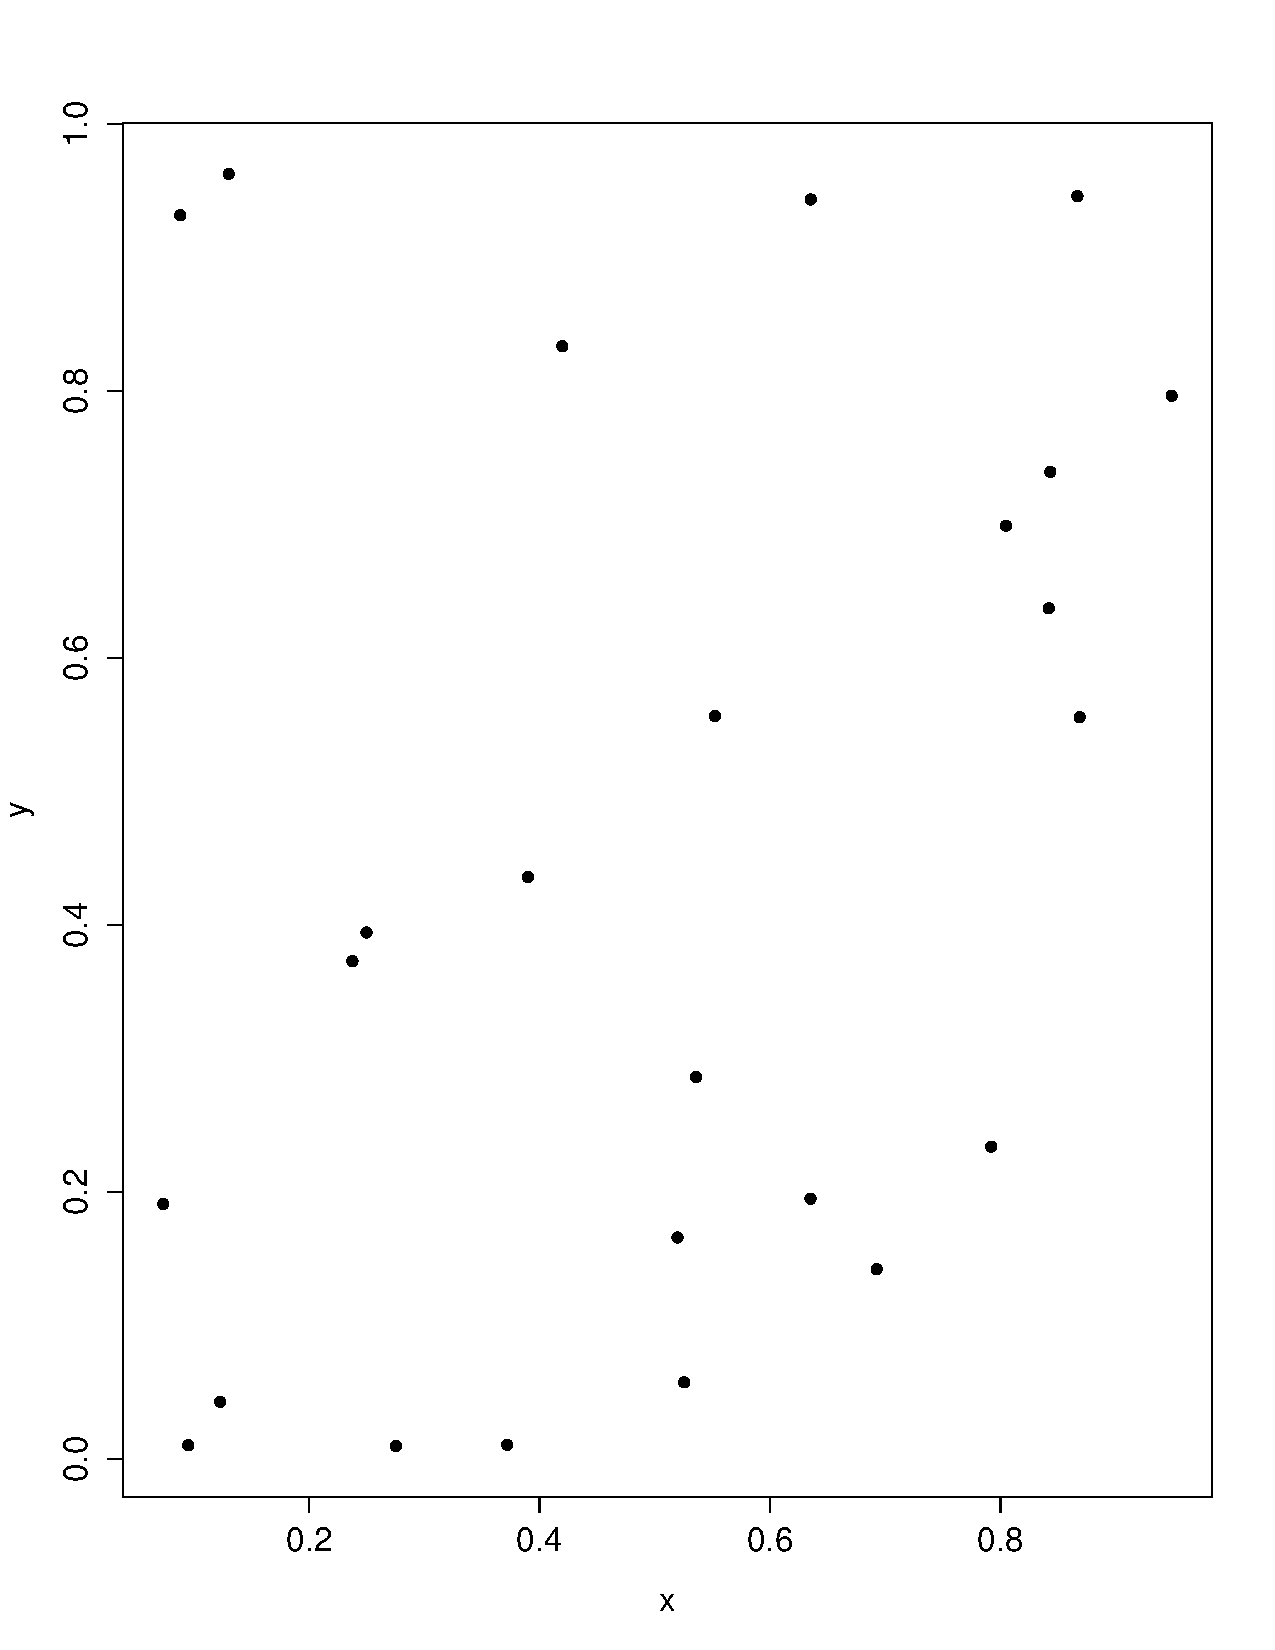
\includegraphics[height = 5cm, width = 6cm]{figure/Bplot.pdf}
  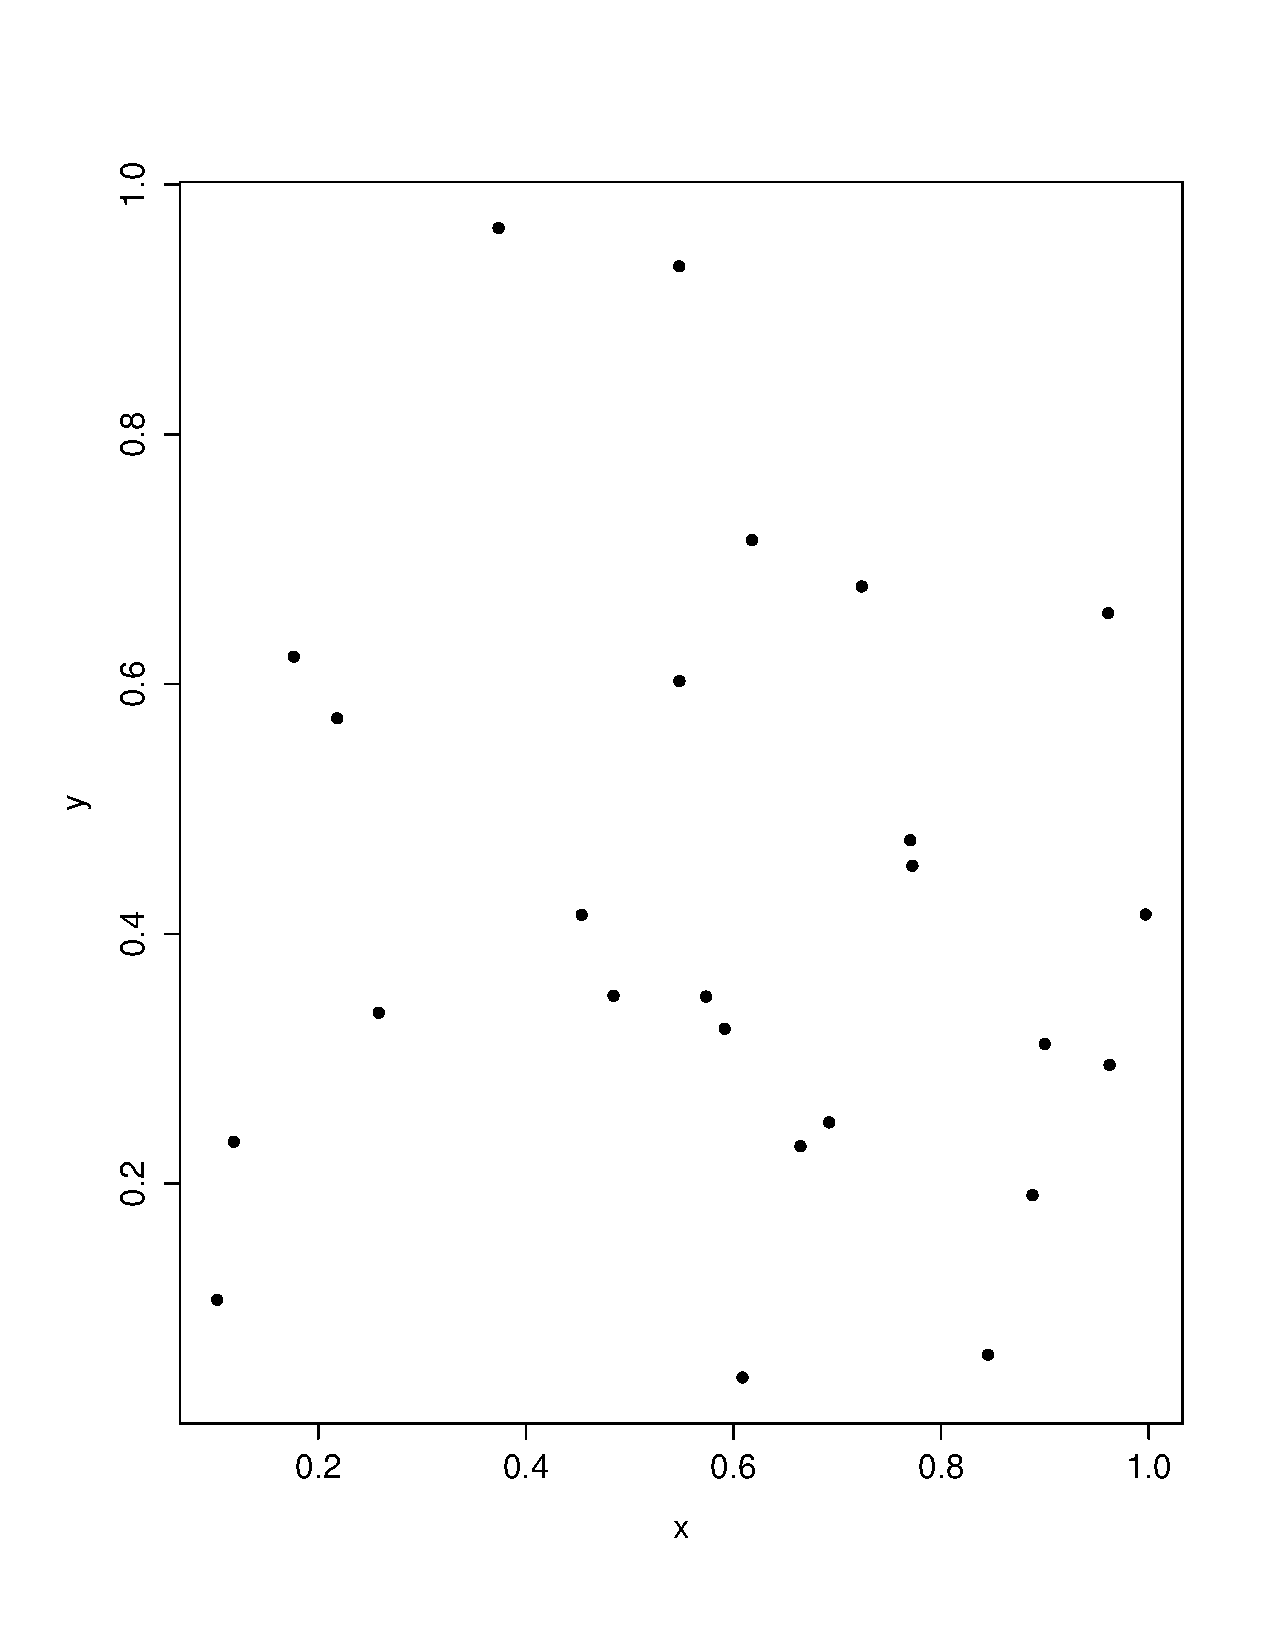
\includegraphics[height = 5cm, width = 6cm]{figure/Gplot.pdf}
  \caption{The left plot drawn by using plot(), the Right plot is redraw it by using grid.echo() on grid graphic system, overall, they are identical to each other(no~~)}
  	\label{figure1}
\end{center}
\end{figure}

\subsection{The problem}
The grid.echo() can replicate most of plot that drawn by the graphics package. However, there are few functions on the graphics package that cannot replicate. One will the the persp() which for drawing 3-dimemtional surfaces. It leads to our aim of this project. Firstable, it is necessary to understand some important theory behind the 3-dimentional plot, such as the transformation from 3-D to 2-D, the drawing order of each ploygons (will be explained later). ect. Then we try to redraw it by using the grid package and we can replicate this function on grid by using the grid.echo().

\begin{figure}[h]
  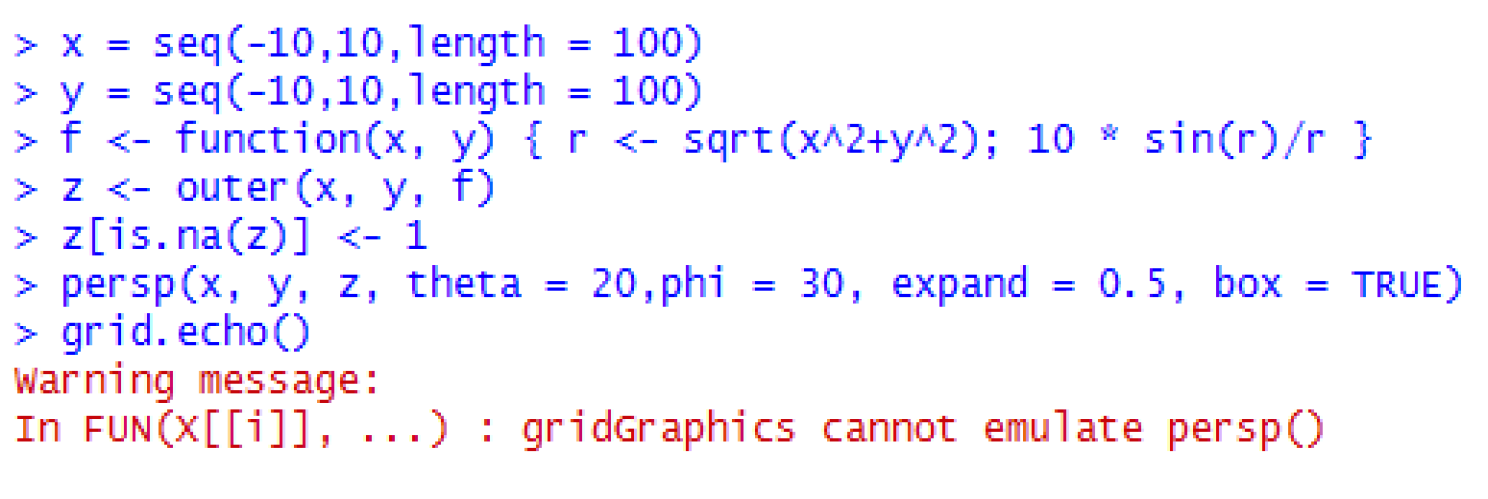
\includegraphics[height = 2.5cm, width = 8.5cm]{figure/warning.png}
  \caption{an example shows that the grid.echo() cannot replicate the persp() on grid}
  	\label{figure2}
\end{figure}

\end{document}
